\chapter{Edge Offloading \& Early Exiting}

Early exiting model have been used for two purposes in literature.

\begin{enumerate}
	\item Reducing average inference latency and power consumption by letting samples prematurely exit the model based on random distributions \cite{bibid} or samples passing a threshold measure of confidence \cite{teerapittayanon_branchynet:_2016}.
	\item Comply with application time constraints by exit selection or sub-model selection. By only inference samples up to a selected exit possible to meet stringent delay constraints and reduce waste of computation \cite{li_edge_2018}. 
\end{enumerate} 

We propose a more flexible edge offloading scheme, compared to upfront exit selection. We argue, that allowing the edge server to reach as far as possible, within the time budget and continuously sending back increasingly confident predictions, will in any case achieve at least the same accuracy. Even though a sub-model exit have been chosen with care, the risk of timeout is still present as both computation and communication delays are not constant. If unexpected delays do occur, it may cause timeouts and lead to lost predictions. However, our scheme reduces the risk of losing prediction by timeout, if an earlier, albeit less accurate predictions is available. 

Figure \ref{fig:offloading-scheme} illustrates the offloading scheme. To not waste idle time on edge server the data is offloaded from the end device, to edge server as soon as acquired. The edge server preprocesses the data, runs the \gls{dnn} inference process, and whenever a prediction is obtained, a thread is spawned to send back the result to the end device. The end device then decides the prediction based upon the information received from the edge server. Figure \ref{fig:offloading-scheme-successful} illustrates the continuous reply of predictions. Figure \ref{fig:offloading-scheme-timeout} illustrates a case, where a timeout occurs and only two predictions are available. 

\begin{figure}
	\captionsetup[subfigure]{justification=centering}
	\subfloat[Continuois predictions\label{fig:offloading-scheme-successful}]{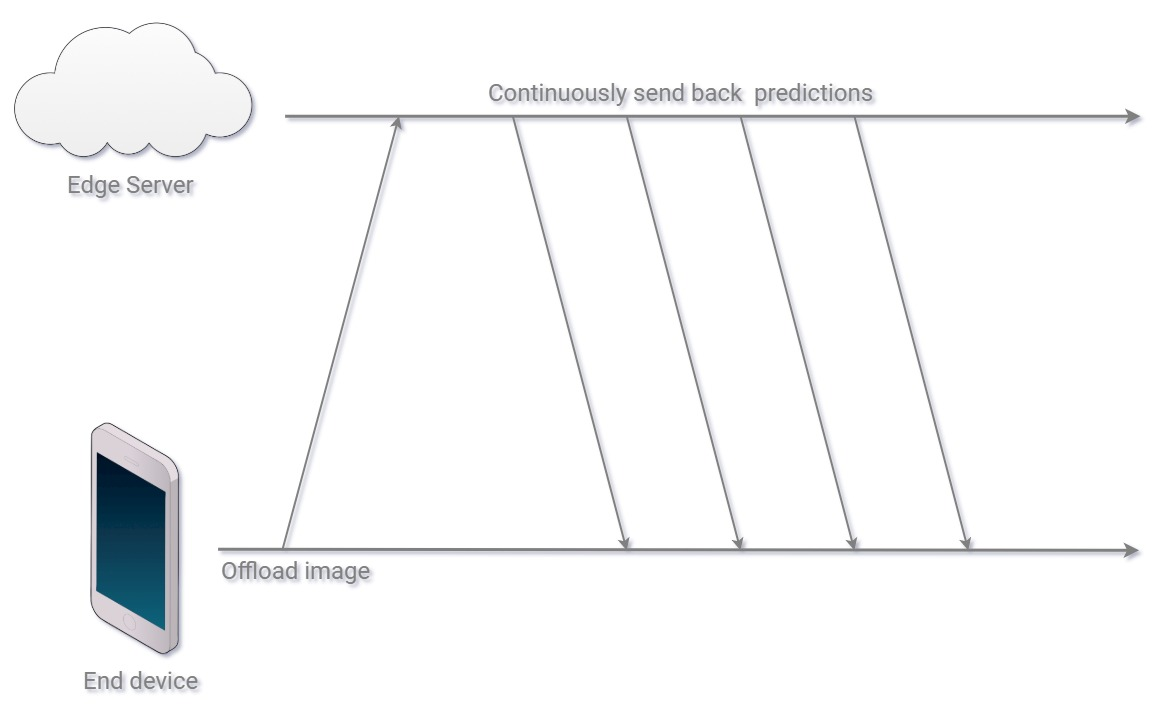
\includegraphics[width=\linewidth]{figures/models/timeline_all}}
	\hfill
	\subfloat[Timeout of Continuois predictions\label{fig:offloading-scheme-timeout}]{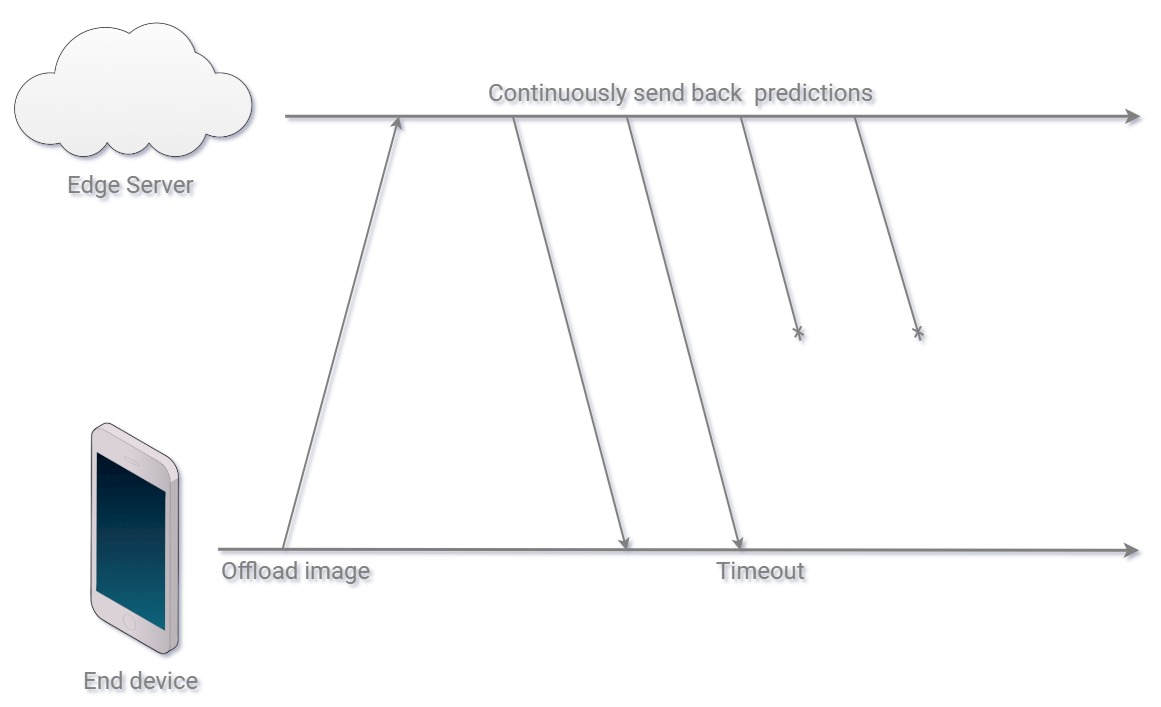
\includegraphics[width=\linewidth]{figures/models/timeline_timeout}}
	\caption[Offloading scheme]{offloading scheme}
	\label{fig:offloading-scheme}
\end{figure} 

\section{Implementation}

The offloading scheme is implemented as a client/server application using the \gls{python} Socket API. The client and server establishes a TCP socket. The client then loads a samples from the \gls{min100} validation set and sends it over the streaming protocol. The server preprocess the sample and runs the model inference. As prediction are obtained a thread is spawned to stream the results back to the end device. 

\section{Experimental Setup}

The client code is deployed on the NUC and server code on the Jetson TX2. The samples and intermediate predictions are timed an logged. 

\section{Results}

Each prediction from received contains two 5-dimensional vectors.  The score vector contains the scores output from the softmax classifier sorted from higest to lowest. The class vector the class labels associated with corresponding score.
\begin{align*}
\mathbf{s}_{exit_n} = \begin{bmatrix}
s_{n,0} & s_{n,1} & s_{n,2} & s_{n,3} & s_{n,4}
\end{bmatrix} \\
\mathbf{c}_{exit_n} = \begin{bmatrix}
c_{n,0} & c_{n,1} & c_{n,2} & c_{n,3} & c_{n,4}
\end{bmatrix}
\end{align*}
Given we receive $n$ prediction within the time frame, we can combine the prediction information by formulating $n \times 5$ matrices S and C.
\begin{align*}
\mathbf{S}_{n,j} = \begin{bmatrix}
s_{0,0} & s_{0,1} & s_{0,2} & s_{0,3} & s_{0,4} \\
s_{1,0} & s_{1,1} & s_{1,2} & s_{1,3} & s_{1,4} \\
\vdots & \vdots & \vdots & \vdots & \vdots \\
s_{n,0} & s_{n,j} & s_{n,j} & s_{n,j} & s_{n,j}
\end{bmatrix} \\
\mathbf{C}_{n,j}= \begin{bmatrix}
c_{0,0} & c_{0,1} & c_{0,2} & c_{0,3} & c_{0,4} \\
c_{1,0} & c_{1,1} & c_{1,2} & c_{1,3} & c_{1,4} \\
\vdots & \vdots & \vdots & \vdots & \vdots \\
c_{n,0} & c_{n,j} & c_{n,j} & c_{n,j} & c_{n,j}
\end{bmatrix}
\end{align*}

\subsection{Exit Score Analysis}

Having multiple predictions available give raise to the question, if we can use the additional information to improve model accuracy? An analysis of data have shown, that the score of an early exit is not always less than a later exit.
\begin{align*}
	S_{exit_{n}} \nless S_{exit_{n+1}}
\end{align*}
Table \ref{tbl:latest-vs-max} show, that simply using the latest exit of the model is lightly better than using the highest scoring among all predictions, as uncertainty is introduced using earlier exits.  

\begin{longtabu}{>{\bfseries}X|X|X}
	\caption[]{} \label{tbl:latest-vs-max} \\
	\toprule
	\rowfont{\bfseries}
	Model & latest exit & max score   \tabularnewline
	\bottomrule
	\endfirsthead
	\multicolumn{3}{@{}l}{\textbf{\textcolor{black}{Table \ref{}:}} continued}\\
	\toprule
	\rowfont{\bfseries}
	Model & $Exit_N$ & max score    \tabularnewline
	\bottomrule
	\endhead % all the lines above this will be repeated on every page
	\bottomrule
	\multicolumn{3}{@{}l}{continued \ldots}\\
	\endfoot
	\hline
	\endlastfoot
	B-Resnet	& 0.8826	& 0.8794  \tabularnewline
	\hline
	B-DenseNet	& 0.8660 	& 0.8602 \tabularnewline 								
	\bottomrule
\end{longtabu}
Figure \ref{fig:exit-highscore} show the distribution of highest scoring exit given the amount of prediction received, and the distribution of samples correctly and incorrectly classified. Looking at the figure added uncertainty can be read directly from highest scoring exit is incorrect, where all predictions are received using the max score one must add the bars from all exits opposed to only using the red bar of $exit_N$. 

\begin{figure}
	\captionsetup[subfigure]{justification=centering}
	\centering
	\subfloat[B-ResNet]{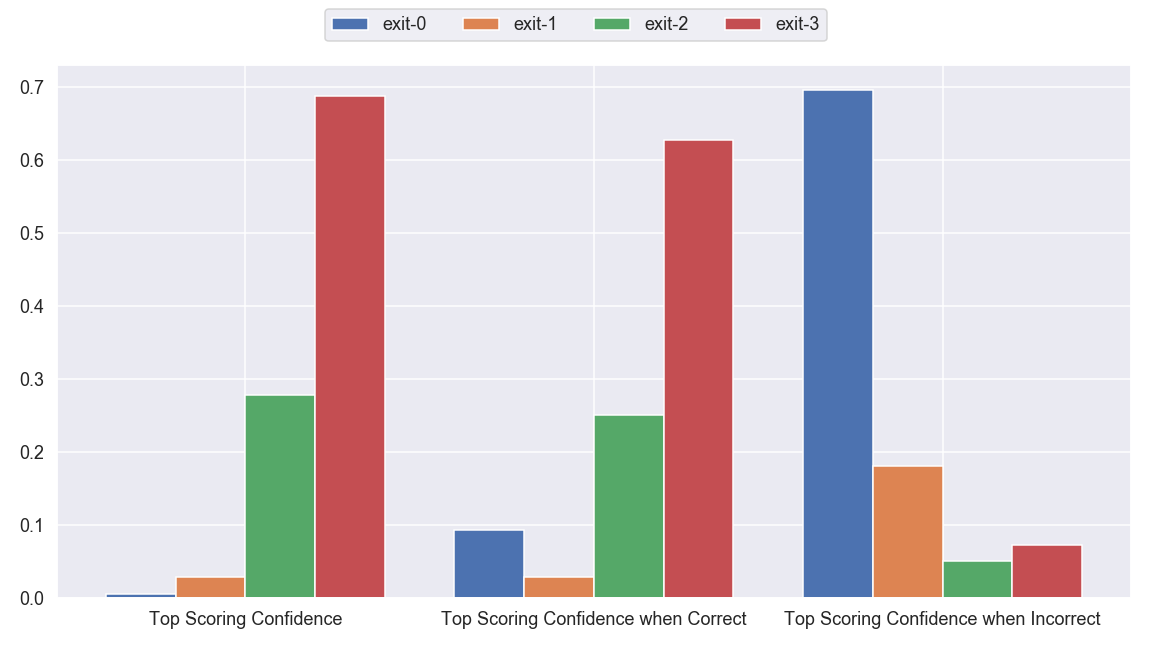
\includegraphics[width=.5\linewidth]{figures/edge/b-resnet_correctness}}
	\hfill
	\subfloat[B-DenseNet]{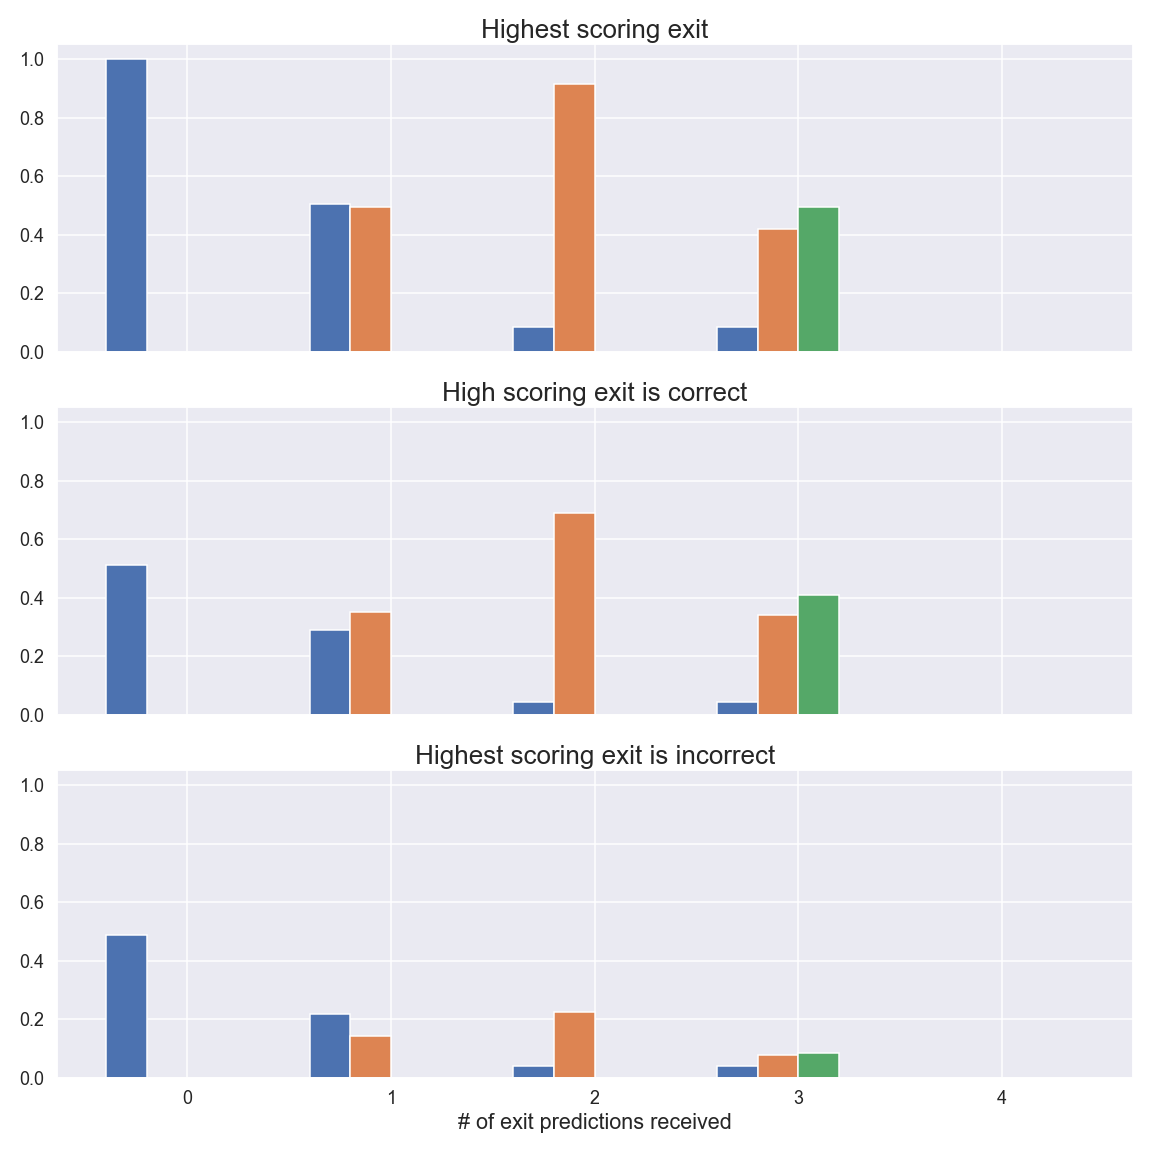
\includegraphics[width=.5\linewidth]{figures/edge/b-densenet_correctness}}
	\caption[short text]{text}
	\label{fig:exit-highscore}
\end{figure}

Yet a study of samples revealed that in some cases an early exit correctly predicted a sample, which a later exit makes incorrect. An example is sample 57, where we denote a prediction vector $\mathbf{p}$ of binary values, where a 1 indicates a correct prediction and 0 the reverse. 
\begin{align*}
\mathbf{p}_{57}=
\begin{bmatrix}
exit_1 \\
exit_2 \\
exit_3 \\
exit_4
\end{bmatrix}
=
\begin{bmatrix}
1 \\
1 \\
0 \\
0
\end{bmatrix}
\end{align*}
Given this insight we define methods to combine the prediction information from multiple exit as efforts to improving the overall model accuracy. 

\subsection{Combining Prediction Information}


We define several proposals for using the additional predictions provided from the early exiting framework, with the purpose to improve the accuracy under time constraints. 

We also examined thresholds in the previous chapter, which did show that a high prediction score, have more chance of being correct.       

\begin{description}
	\item[Last Exit] We define the method \emph{last exit}, where we constraint ourselves to only use the most recent prediction $n$, where we find the concrete prediction $p$ as the highest scoring class. 
	\begin{align*}
		p = \mathbf{c}_{n, \arg \max  \mathbf{s}_n} = c_{n,0}
	\end{align*}
	 Choosing the most confident prediction from the most recent result available, gives us the highest accuracy on average. However, we only use information form a single prediction, we might be able to formulate a mathematical function able to use information form multiple predictions to further improve the accuracy, as we have seen, that the later exit might make a correct prediction from an earlier exit incorrect. 
	 
	\item[Confidence (max)] This method is based on the naive assumption, that given a higher score, it will lead to a higher accuracy independent of the uncertainty of classifier at the exits. We use all available predictions, and choose the most confident one, i.e. the one with the highest score.
	\begin{align*}
	p = \mathbf{C}_{\arg \max  \mathbf{S}}
	\end{align*}
	Here we neglect the fact, that the later exits are in general more accurate and assume, that a higher confidence despite the exit leads to a correct prediction and we do not account for the uncertainty introduces be less accurate exits.
	\item[Score-margin (max)] We consider all available results and determines the score-margin between the two top-scoring predictions. We select the prediction from the exit with the highest score-margin. From the previous chapter, we know that the score-margin threshold gave a smaller proportion of incorrrectly exited samples at the small cost of samples, that could have been correctly classified using only highest scoring confidence.
	
	\item[Confidence (add)] We define a method, that additive combines all information from all available predictions and selects the highest scoring class. The returned vectors from the prediction is a sparse representation of class labels and a vector associated scores, which may contain different classes for predictions from different exits. In order to combine the information by addition the vector must be expanded back to the original class space with $k$ classes. For the \gls{min100} $k=100$. We pad zeros between all missing class labels for the score vectors $\mathbf{s}_{exit_n}$. Thus, after expansion the vector only have non-zero values at the top-5 prediction indices.
	\begin{align*}
		\mathbf{s}_{exit_n} = 
		\begin{bmatrix}
			s_{n,0} & \dots s_{n,4}
		\end{bmatrix}_{1 \times 5} 
		\xrightarrow{expand} 
		\begin{bmatrix}
		s_{n,0} & \dots & s_{n,k-1}
		\end{bmatrix}_{1 \times k,\: k=100} 
	\end{align*}
	After expansion the class vector $\mathbf{c}$ contains all class labels ordered and of course becomes identical for all exits.
	\begin{align*}
		\mathbf{c}_{exit_n}= 
		\begin{bmatrix}
		c_{n,0} & \dots & c_{n,4}
		\end{bmatrix}_{1 \times 5}
				\xrightarrow{expand} 
		\mathbf{c} =
		\begin{bmatrix}
		0 & \dots & k-1
		\end{bmatrix}_{1 \times k,\: k=100} 
	\end{align*}
	
	 Now that the ordering of classes and scores are on standard form, we can use the matrix notation and sum all columns of the score matrix to construct a new combined score vector $\mathbf{s^*}$.
	\begin{align*}
		\mathbf{s^*} = \sum_{i=0}^{k} \mathbf{s}_{n,i}, \text{for\:} n=0, 2, \dots, j =		
		\begin{bmatrix}
		s^*_0 & s^*_1 \dots & s^*_{k-1}
		\end{bmatrix}_{1 \times k,\: k=100} 
	\end{align*}
	The prediction becomes the class with the highest value in $\mathbf{s^*}$
	\begin{align*}
		\mathbf{p} = C_{\arg \max \mathbf{s^*}}
	\end{align*}
		
	\item[Score-margin (add)] Similarly we define a method, that determines the score-margin using the two highest scoring classes from each prediction and additive combines the informations.
	\item[Confidence (add,weight)] Almost identical to \emph{confidence (add)}, but uses a weighted sum of all available exits to combine the information. The weights can be represented by a column vector $\mathbf{w}$.
	\begin{align*}
		\mathbf{w}_{exit_n} =
		\begin{bmatrix}
			w_0 \\
			w_1 \\
			\vdots \\
			w_j
		\end{bmatrix}
	\end{align*}
	Each exit are weighted to acknowledge the increasing accuracy as the predictions comes from a deeper exit in the model. The output is still a $k$-dimensional vector representing the score for each class. 
	\begin{align*}
	\mathbf{s^*} = \sum_{i=0}^{k} w_n \cdot \mathbf{s}_{n,i} , \text{for\:} n=0, 2, \dots, j = 		
	\begin{bmatrix}
	s^*_0 & s^*_1 \dots & s^*_{k-1}
	\end{bmatrix}_{1 \times k,\: k=100} 
	\end{align*}
	The prediction becomes the class with the highest value in $\mathbf{s^*}$
	\begin{align*}
	\mathbf{p} = C_{\arg \max \mathbf{s^*}}
	\end{align*}
	
	\item[Score-margin (add,weight)] Similarly we define a weighted sum version of the score-margin. 
\end{description}

\begin{figure}
	\centering
	\subfloat[subcaption]{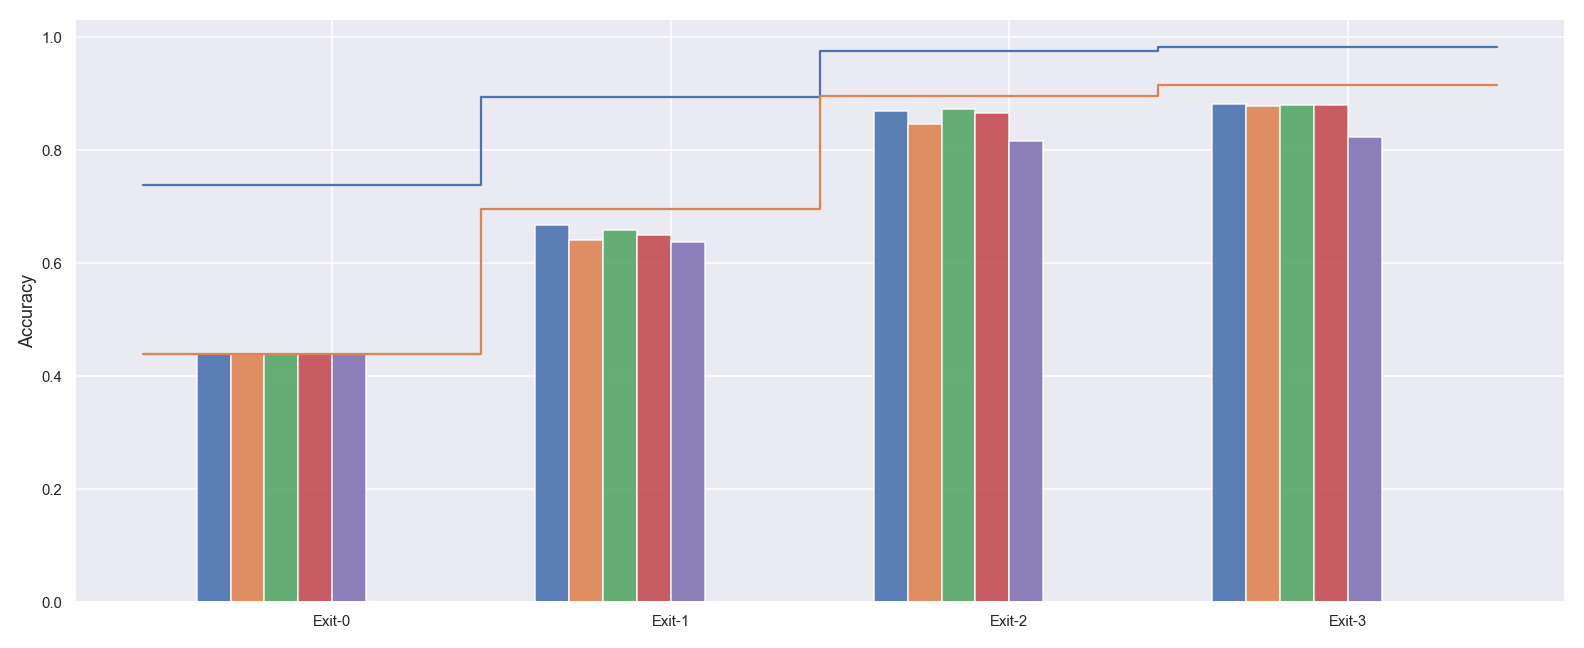
\includegraphics[width=.7\linewidth]{figures/edge/b-resnet_theoretical_score_combinations}}
	\hfill
	\subfloat[subcaption]{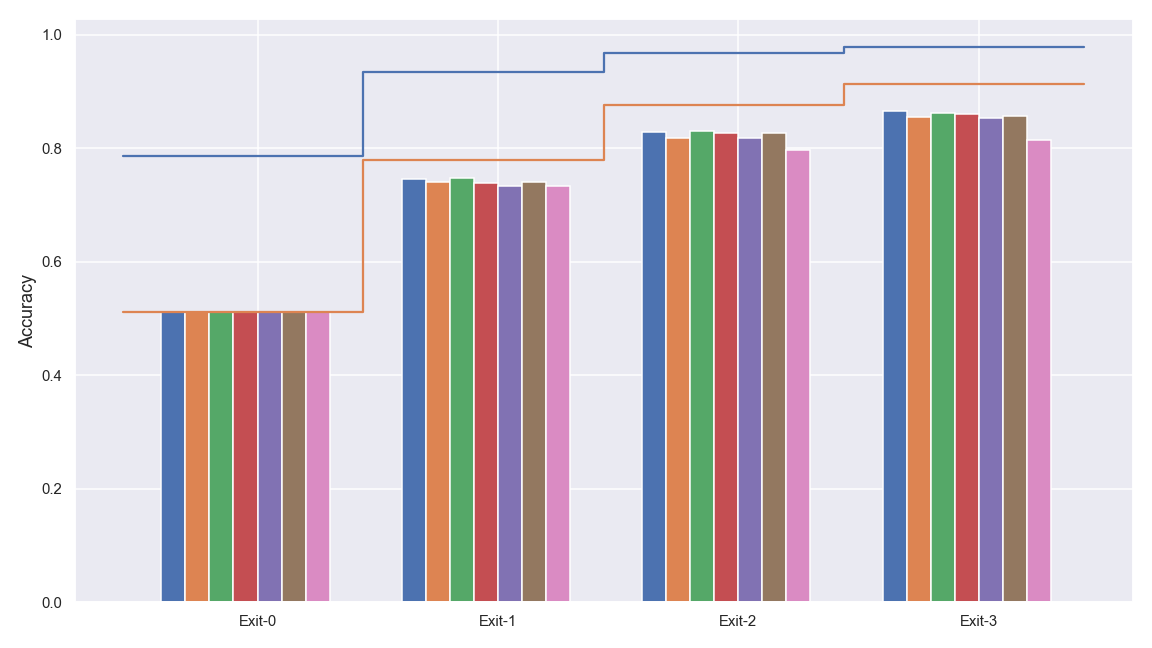
\includegraphics[width=.7\linewidth]{figures/edge/b-densenet_theoretical_score_combinations}}
	\caption[short text]{text}
	\label{fig:info-combi}
\end{figure}

The blue line optimum-top5 show the maximum achievable accuracy, if we were always able to pick the right class among the top5 predictions given the number of exit results received. The orange line optimum-top1 show the optimal line if, we were always able to pick the correct class among the top1 prediction given the number exit results received.

\subsection{Delay Constraint}

How far are we able to in inference process under different time constraints? 

\begin{figure}
	\centering
	\subfloat[]{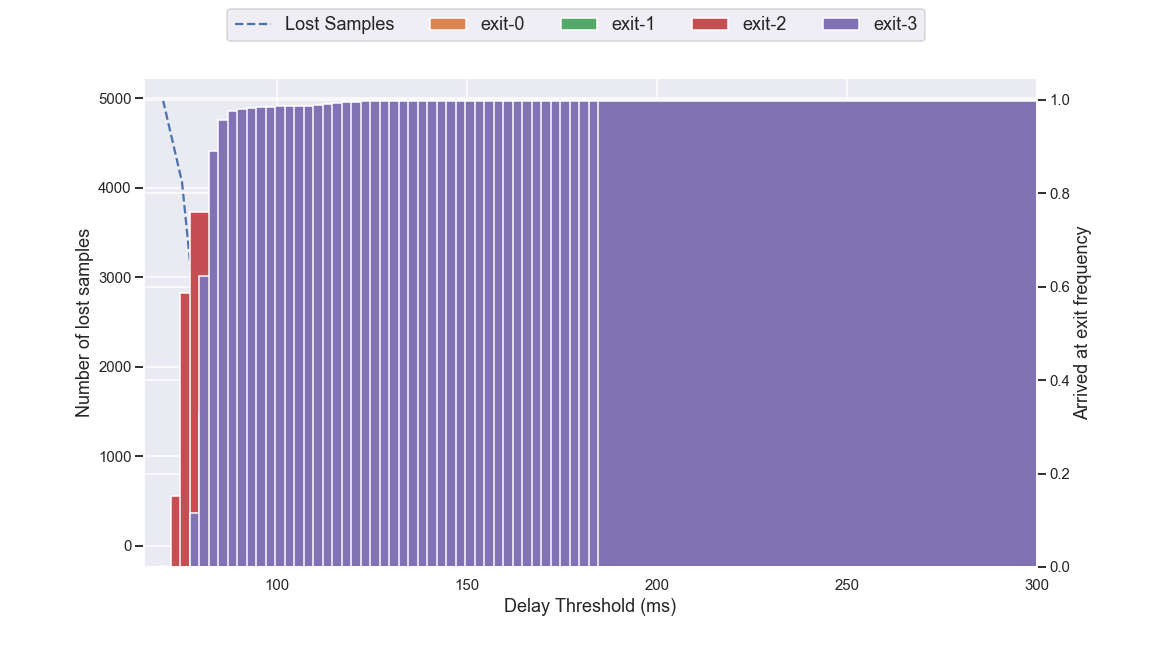
\includegraphics[width=.7\linewidth]{figures/edge/b-resnet_exit-reached}}
	\hfill
	\subfloat[]{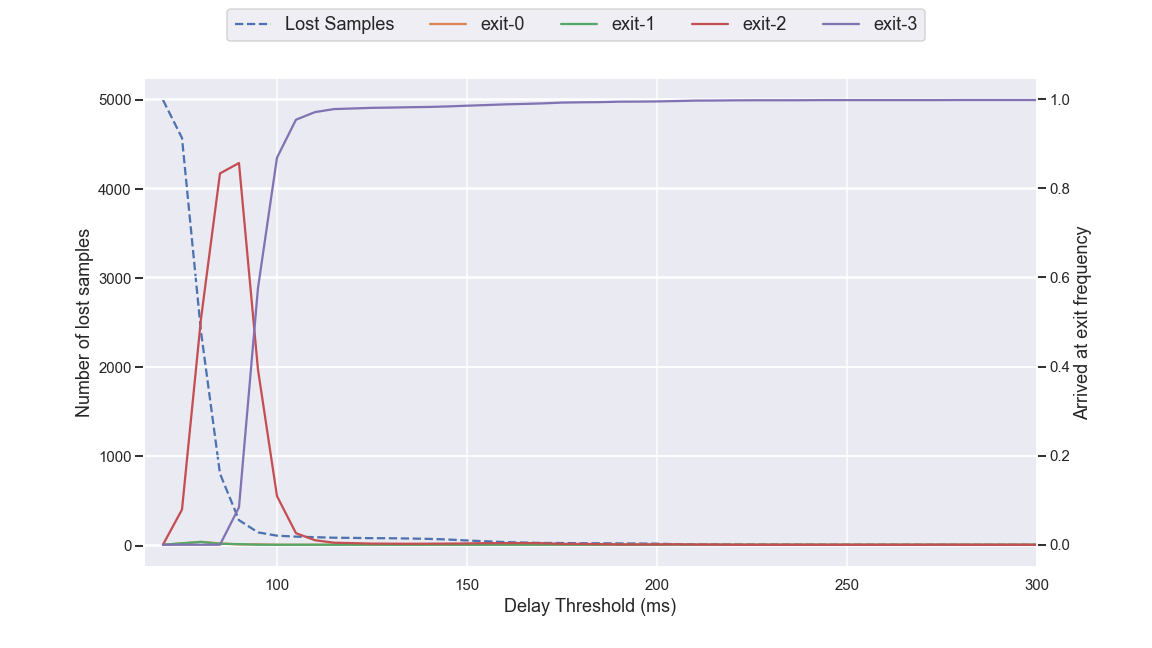
\includegraphics[width=.7\linewidth]{figures/edge/b-densenet_exit-reached}}
	\caption[short text]{text}
	\label{fig:exit-reached}
\end{figure}

\begin{figure}
	\centering
	\subfloat[subcaption]{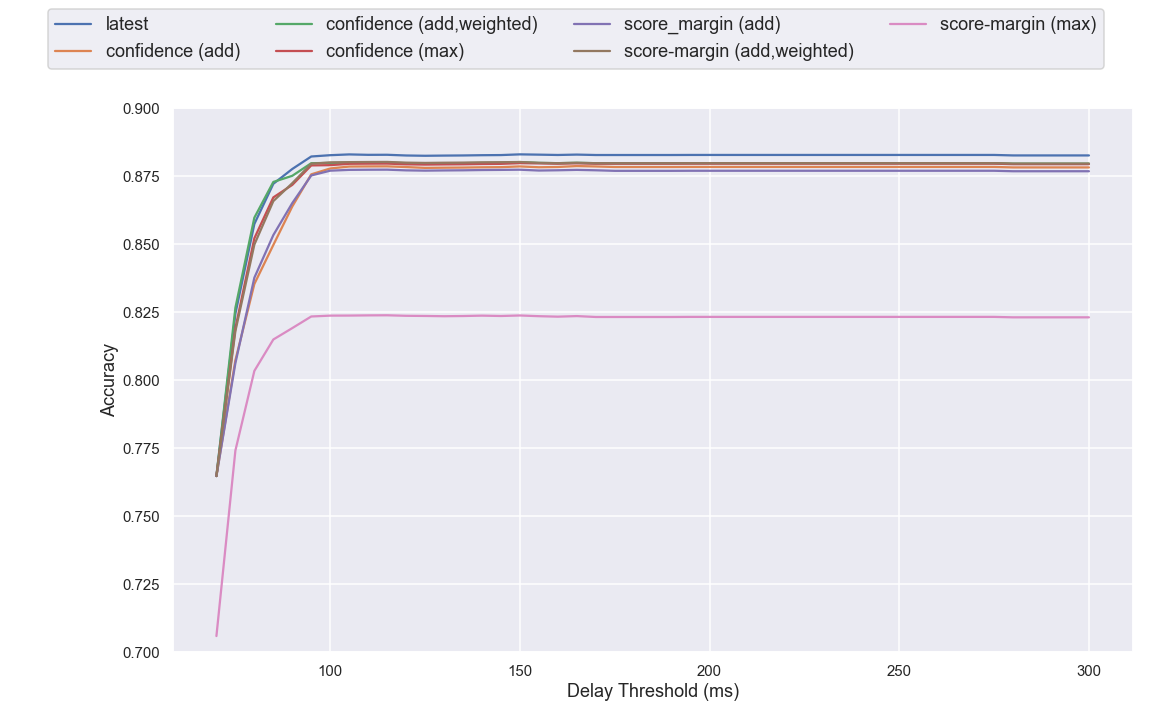
\includegraphics[width=\linewidth]{figures/edge/b-resnet_information-combination.png}}
	\hfill
	\subfloat[subcaption]{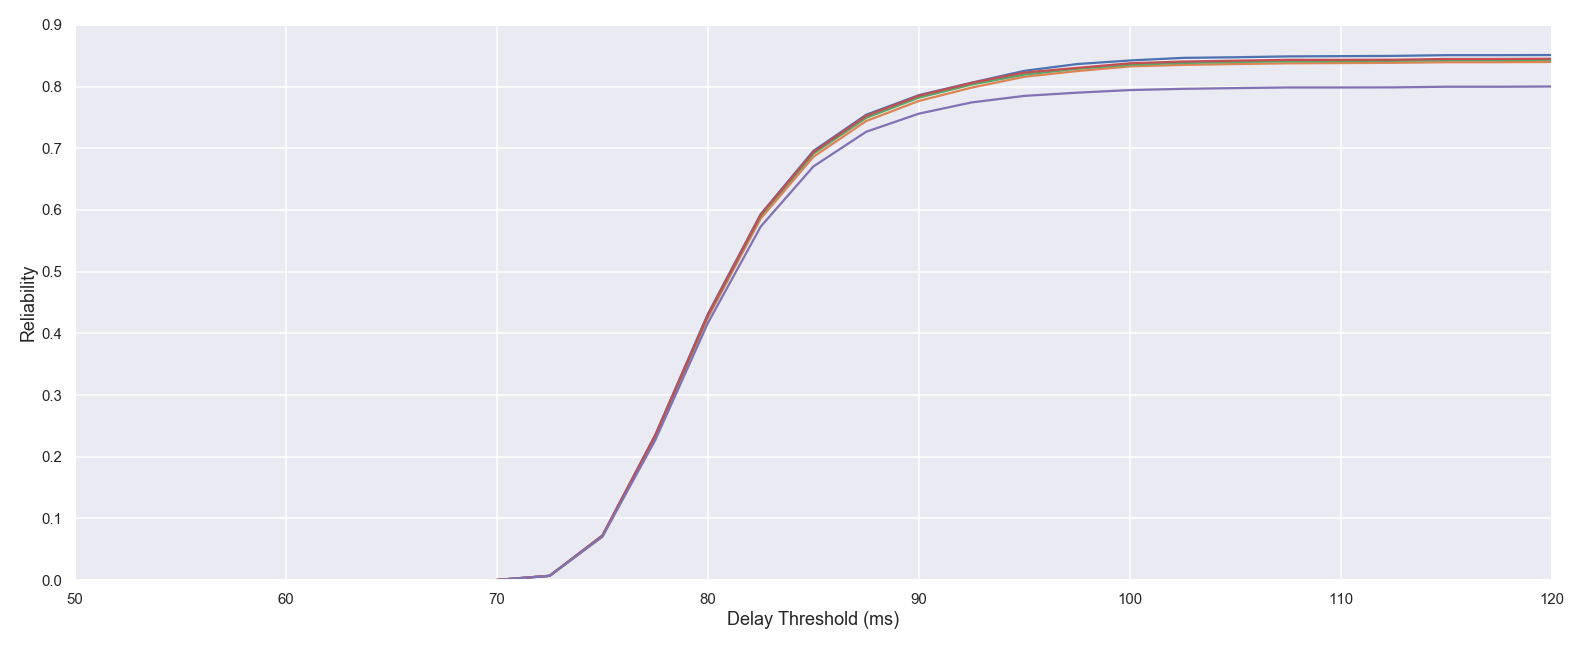
\includegraphics[width=\linewidth]{figures/edge/b-densenet_information-combination.png}}
	\caption[short text]{text}
	\label{fig:info-combi}
\end{figure}

Should I create hybrid combinations? Maybe only combine info from exit-0 and -1 and always let exit-2 and -3 have the final say if available? What if we can combine info from those two and omit the poor ones? 


\subsection{Transport Protocol} 

Offloading tasks over the network, irregardless fully or partially requires a transport protocol. The selection is typically a choice of either \gls{tcp} or \gls{udp}. \gls{tcp} is a reliable protocol, that guarantee no losses by retransmission of lost packets. \gls{udp} on the other hand is a best-effort protocol, that accept packets loss, thus not introducing retransmission communication overhead. 


Fully offloading \gls{jpeg} compressed images for classification require no losses for human-readability. Sending intermediate features of a \gls{dnn} may not be as intolerant to losses and might be able to function with the far more lightweight \gls{udp}. In current research literature the choice of \gls{tcp} seems given in advance.  

In this experiment the \gls{tcp} transmission time and retransmission rate is investigated under different communication environments. 

\begin{figure}
	\centering
	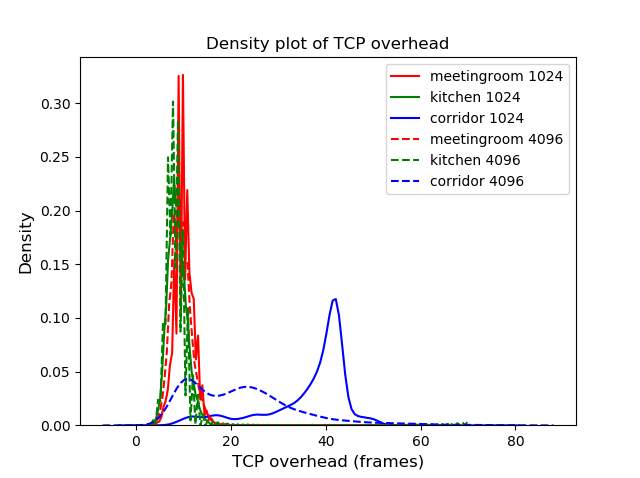
\includegraphics[width=\linewidth]{figures/tcp/tcpoverhead}
	\caption[TCP retransmission overhead]{TCP retransmission overhead}
\end{figure}